\chapter{\cink{} semantics for restrict}\label{chap:cink}
In chapter \ref{chapter:examples}, we have given an intuition for the semantics of restrict and how
compilers exploit the information it provides.
In this chapter, we will discuss the fragment of the \cink{} semantics for restrict.
Based on an analysis of the K-sources\footnote{Available at \url{https://github.com/kframework/c-semantics/tree/master}}, the generated \textsc{kcc} interpreter
and an additional unpublished paper (an elaborate version of Hathhorn \etall \cite{hathhorn2015defining}), we redeveloped their semantics in a functional style and found
several issues.

In section \ref{sec:memory-model} we give some background information on memory models for C and their design considerations.
In section \ref{sec:restrict-sem} we present and explain the functional \cink{} semantics.
Finally, section \ref{sec:cink-incorrect} argues why some aspects of the semantics are incorrect
with respect to the standard.
We note that there are several representational discrepancies for either simplification or adaption 
of the functional style implementation, of which a complete overview can be found in related work section \ref{sec:representational-discrepancies}. 

\section{Memory model}\label{sec:memory-model}
In order to define a semantics for a language such as C, one needs to model the memory to reflect how allocations, stores and other operations affect the ``memory state" of the abstract machine.
The design of such a model is quite a crucial aspect for a C semantics, because more sophisticated models are able to catch various cases of undefined behavior.
As a result there exist many variations of memory models, which can be classified as being concrete, abstract or somewhere in between (hybrid) \cite{leroy2008formal, memarian2019exploring}.

A typical \textit{concrete} model, such as the one used by Norrish \cite{norrish1998c}, is defined as $\Memvar \in \textit{Mem}_\textit{concrete} := [0, 2^n) \rightarrow [0, 256)$,
with $n$ being the size of the address space.
This type of model is closest to how an actual computer works, \ie addresses are numerical values which map to integer values
between 0 and 256.

A typical \textit{abstract} model was created for the CompCert project by Leroy \etall \cite{leroy2012compcert}.
It is defined as $\Memvar \in \textit{Mem}_\textit{abstract} := \Loc \rightarrow \Val$, thus moving away from the underlying numerical representations.
Locations are defined as $\Locvar \in \Loc := \Block \times \Offset$, with $\Blockvar \in \Block$ being a reference to the memory block and $\delta \in \Offset$ the byte offset into the block.
Values are defined as $\Valvar \in \Val \ \bnfdef \ [0, 256) \ | \ \mathconstr{Ptr}(\Locvar, m) \ | \ \vundef$, denoting
integer values, pointer fragment $m$ of location $\Locvar$ and uninitialized values.
The \cink{} memory model is based on this model.
We use the term \textit{provenance}, going back to at least Defect Report \#260 \cite{defect260},
to describe the extra information of a pointer value, which is used to distinguish it from another pointer value that would
have an equivalent numerical value under a concrete memory model.
For example, tracking block references is a form of provenance to determine from which memory block
a location is derived.

We stated that an abstract model can capture more undefined behavior than a concrete one.
An example of undefined behavior which is captured by the CompCert memory model is
out of bounds pointer arithmetic.
In C it is illegal to access memory locations via pointer arithmetic, if the arithmetic expression would point into
another object than the pointer operand \cite[6.5.6]{ISO:2018:III}.
Because memory blocks are separated by construction in CompCert, this restriction is directly captured
as arithmetic with pointers only changes the location offset (making it impossible to change the block reference).
For example, consider the function \texttt{problematic} below.
It compares the addresses \texttt{\&x + 1} and \texttt{\&y}, 
which could evaluate to true if an implementation allocated \texttt{x} and \texttt{y} adjacent to each other.
Under the CompCert memory model it is straightforward to give undefined behavior, because the pointer arithmetic
would result in a location outside the object bounds of \texttt{x}.

\begin{code}
\begin{minted}[escapeinside=||,mathescape=true,linenos]{c}
void problematic()
{
    int x, y;
    if (&x+1 == &y) { // Illegal pointer arithmetic
        ...
    }
}

\end{minted}
% \caption{Pointer arithmetic into a different object}
% \label{lst:example-separated-by-construction}
\end{code}

An example of a limitation of the abstract model is that it is not possible to use memory addresses as integers, \eg for pointer to integer casts.
A \textit{hybrid} model, such as the PVI and different PNVI models by Memarian \etall \cite{memarian2019exploring, sewellc}, combines aspects of 
concrete and abstract models by giving meaning to casts between pointer and integer values while also tracking provenance. 

\section{Restrict semantics}\label{sec:restrict-sem}
The \cink{} semantics has two features which are jointly used to support restrict.
Pointer values have a provenance called \textit{bases}, which is used to track from which
restrict qualified objects they are derived (1).
For each location a restrict state is tracked that says which memory accesses are allowed and which are not (2).
For feature (2) there is a structure of a stack (called the \textit{restrict stack}) to track the restrict states 
and of a lattice which defines allowed and disallowed accesses.

By means of the preliminary grammar of figure \ref{fig:cink-domains} we introduce the
domains and types necessary for explaining the restrict features of the \cink{} semantics in detail.
The semantics itself will then be explained by elaborating on some example programs.

\begin{figure}[htb]
\[\def\arraystretch{1.1}
\begin{array}{lrll}
    b \in \Block, \delta \in \Offset            &   :=          & \Intdomain                                                      & \\
    \Scopeidvar \in \Scopeid                    &   :=          & \Intdomain                                                      & \\
    \Simplelocvar \in \Simpleloc                &   :=          & \Block \times \Offset                                           & \\
    \Basevar \in \Base                          &   :=          & \Block \times \Scopeid                                          & \\
    \Basesvar \in \Bases                        &   :=          & \Set{\Base}                                                     & \\
    l \in \Loc                                  &   :=          & \Simpleloc \times \Bases                                        & \\
    \Restrictstatevar \in \Restrictstate        &   \bnfdef     & \onlyread{\Basesvar}                                               & \\
                                                &   |           & \restricted{\Basesvar}                                             & \\
                                                &   |           & \unrestricted                                                   & \\
                                                &   |           & \rsub                                                           & \\
                                                &   |           & \bot                                                            & \\
    \Restrictmapvar \in \Restrictmap            &   :=          & \Simpleloc \rightharpoonup \Restrictstate                           & \\
    R \in \Restrictstack                        &   :=          & \List{\Scopeid \times \Restrictmap}                             &
\end{array}
\]
\caption{\cink{} restrict related domains}
\label{fig:cink-domains}
\end{figure}

Programs in the \cink{} semantics are evaluated under a restrict stack $R$, which is modified through scope changes 
and memory accesses.
Locations \Locvar \ are represented by tuples, whose first component \Simplelocvar \
is the memory location composed of a block reference and offset pair (based on CompCert \cite{leroy2012compcert}).
The second component of \Locvar \ is a set of \Bases \
\Basesvar, whose elements $\Basevar$ are tuples $(\Blockvar, \Scopeidvar)$ in which $\Blockvar$ represents the block reference
of the restrict qualified object $p$
from which \Locvar \ is derived and $\Scopeidvar$ the unique identifier of the scope in which $p$ was declared.
It is a \textit{set} since restrict pointers may be assigned to each other, if the pointer being assigned to is declared in a nested scope\footnote{This corresponds to example 4 of the section on restrict in the standard \cite[6.7.3.1]{ISO:2018:III}}.

We say that a location (or the location an lvalue exression is stored at) $(\Simplelocvar, \set{\dots, (\Blockvar, \_), \dots})$
is \textit{derived from} a restrict qualified object $b$ if it is obtained through 
a dereference of a pointer expression which is \textit{based on} $b$.
For example, given the following code snippet \mintinline{c}{int x; int* restrict p = &x;} we have that the expression $*p$ is
derived from the restrict qualified object $p$ because $p$ is based on $p$, but $\&x$ is not derived from $p$.

The memory relates \Simpleloc s to values and will be formally defined when we present the complete
language in section \ref{section:syntax}.
Importantly, every variable has an address in memory in order to support the address of (\&) operator.
We write $\Memvar(\Simplelocvar)$ to denote the value stored at $\Simplelocvar$, at the execution point
the annotation is placed at.
Pointer values are denoted as $\ptr{(\Simplelocvar, \Basesvar)}$, \ie they contain a \Loc, with $\Simplelocvar$ being
the location pointed towards and \Basesvar \ the provenance of the pointer value.
The aim of \Basesvar \ is to track the \textit{based on} definition we previously explained in chapter \ref{chap:introduction} and section \ref{section:iso-definition}.

An example of how the set of bases transforms through assignments is given in listing \ref{lst:example-based-on}.
In this example, a restrict pointer $p$ is created to the variable $x$ at line \ref{lst:example-bases-line-p}.
The value of $p$ is not just the $\Simpleloc \ \Simplelocvar_x $ representing $x$'s address,
but also the base $(\Blockvar_p, \scope{main})$ to track that $p$ is based on $p$.
The call to $\mathtt{foo}$ at line \ref{lst:example-bases-line-call} then shows how a location can have multiple bases: the value of $q$ preserves the existing provenance but also becomes derived from the restrict pointer $q$.
After adding this new base, the pointer value of $q$ now has the following provenance: $\set{(b_p, \scope{main}), (b_q, \scope{foo})}$.

The restrict stack $R$ contains tuples of scope identifiers $\Scopeidvar$ and restrict maps $\Restrictmapvar$ from simple memory locations $\Simplelocvar$ to 
a restrict state $\Restrictstatevar$.
This map is used as a total function $\Simpleloc\rightarrow \Restrictstate$ by the following definition: 
$\Restrictmapvar(\Simplelocvar) = \Restrictmapvar(\Simplelocvar)$ if $\Simplelocvar$ is a key in $\Restrictmapvar$, and $\bot$ otherwise.
A tuple $(\Scopeidvar, \Restrictmapvar)$ is pushed onto the restrict stack when the program enters a new scope \Scopeidvar \ and
popped off the restrict stack when a scope is exited.
Consequently, the top item of $R$ always represents the deepest scope that is currently active.

Whenever a program accesses a memory location $(\Simplelocvar, \Basesvar)$
the restrict state representing the access type ($\onlyread{\Basesvar}$ for loads and $\restricted{\Basesvar}$ for stores)
is attempted to be \textit{joined} with the current restrict state of $\Simplelocvar$ in the top restrict map of $R$.
The symmetric join ($\joinsym$) operator (defined in figure \ref{fig:auxiliary-join}) determines what the new restrict state of $\Simplelocvar$ in this map after the join is.
If a join resulted in $\mathconstr{Unrestricted}$, multiple loads from a location occurred within the same scope but the location provenance (\ie bases) differed.
This means the program may now only load from this location (with any pointer) and stores are completely forbidden.
If a join resulted in \rsub, the accesses have violated the semantics of restrict and the program has undefined behavior.
As a result the program execution is aborted and an error is returned.

\newpage

\begin{code}
\begin{minted}[escapeinside=||,mathescape=true,linenos]{c}
// Scope $\scope{foo}$
void foo(int* restrict q) { // $q$ is stored at $\Simplelocvar_q = (b_q, 0)$
    ...                     // $M(\Simplelocvar_q) = \ptr{(\Simplelocvar_x, \set{(b_p, \scope{main}), (b_q, \scope{foo})})}$
}

// Scope $\scope{main}$
int main() {
    int x = 0;              // $x$ is stored at $\Simplelocvar_x$
    int* restrict p = &x;   // $p$ is stored at $\Simplelocvar_p = (b_p, 0) \label{lst:example-bases-line-p}$
                            // $M(\Simplelocvar_p) = \ptr{(\Simplelocvar_x, \set{(b_p, \scope{main})})}$
    foo(p);                 // The value of $p$ is passed to $q$ $\label{lst:example-bases-line-call}$
    return 0;
}

\end{minted}
\caption{Designating and transferring bases provenance}
\label{lst:example-based-on}
\end{code}

\begin{figure}[h]
\centering
\begin{minipage}{.55\textwidth}
    \centering
    \begin{alignat*}{3}
    \onlyread{\Basesvar}    & \joinsym \ & \onlyread{\Basesvar}   = \   & \onlyread{\Basesvar} \\
    \onlyread{\Basesvar}    & \joinsym \ & \restricted{\Basesvar} = \   & \restricted{\Basesvar} \\
    \restricted{\Basesvar}  & \joinsym \ & \restricted{\Basesvar} = \   & \restricted{\Basesvar} \\
    \onlyread{\Basesvar}    & \joinsym \ & \onlyread{\Basesvar'}  = \   & \unrestricted  \\
    \onlyread{\Basesvar}    & \joinsym \ & \unrestricted   = \          & \unrestricted \\
    \unrestricted           & \joinsym \ & \unrestricted   = \          & \unrestricted \\
    \onlyread{\Basesvar}    & \joinsym \ & \restricted{\Basesvar'} = \  & \rsub \\
    \restricted{\Basesvar}  & \joinsym \ & \restricted{\Basesvar'} = \  & \rsub \\
    \restricted{\Basesvar}  & \joinsym \ & \unrestricted   = \          & \rsub \\
    \textit{lhs}            & \joinsym \ & \rsub        = \             & \rsub \\
    \bot                    & \joinsym \ & \textit{rhs}    = \          & \textit{rhs}  \\
    \end{alignat*}
\end{minipage}%
\begin{minipage}{.45\textwidth}
    \centering
    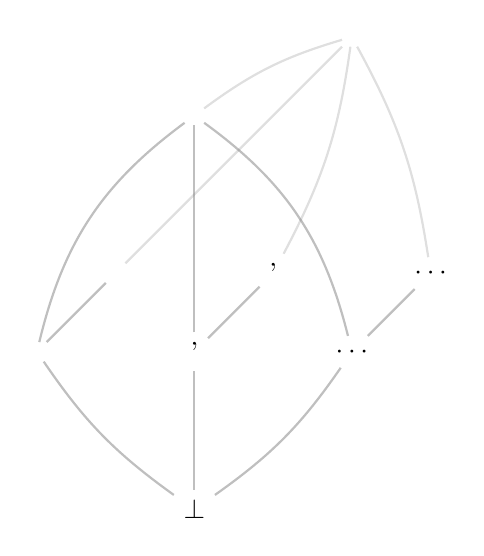
\begin{tikzpicture}
        \node (ub)     at (7,5) {\rsub};
        \node (un)     at (5,4) {\unresabbr};
        \node (rsbs)   at (4,2) {\resabbr{\Basesvar}};
        \node (rsbs')  at (6,2) {\resabbr{\Basesvar'}};
        \node (rsbs'') at (8,2) {$\cdots$};
        \node (orbs)   at (3,1) {\orabbr{\Basesvar}};
        \node (orbs')  at (5,1) {\orabbr{\Basesvar'}};
        \node (orbs'') at (7,1) {$\cdots$};
        \node (bot)    at (5,-1) {$\bot$};

        \path[thick, black, opacity=0.25]
        (bot) edge[bend left=10] node {} (orbs)
        (bot) edge node {} (orbs')
        (bot) edge[bend right=10] node {} (orbs'')
        
        (orbs) edge node {} (rsbs) 
        (orbs') edge node {} (rsbs')
        (orbs'') edge node {} (rsbs'')  
        
        (orbs) edge[bend left=20] node {} (un)
        (orbs') edge node {} (un)
        (orbs'') edge[bend right=20] node {} (un)
    
        (rsbs) edge[gray] node {} (ub)
        (rsbs') edge[bend right=10, gray] node {} (ub)
        (rsbs'') edge[bend right=10, gray] node {} (ub)
    
        (un) edge[bend left=10, gray] node {} (ub);
    \end{tikzpicture}
\end{minipage}
\caption{Auxiliary symmetric operation $\joinsym$ which joins two restrict states, where $\Basesvar \neq \Basesvar'$
            and the corresponding Hasse diagram of the set {\small $\set{\rsub, \unresabbr = \unrestricted, 
            \resabbr{\Basesvar} = \restricted{\Basesvar}, \resabbr{\Basesvar'} = \restricted{\Basesvar'},
            \orabbr{\Basesvar} = \onlyread{\Basesvar}, \orabbr{\Basesvar'} = \onlyread{\Basesvar'}, \bot}$} }
\label{fig:auxiliary-join}
\end{figure}

\begin{figure}[htp]
\begin{align*}
\filterbases                                      : & \ RestrictState \times ScopeId \rightarrow RestrictState \\
\filterbases \ (\onlyread{\Basesvar}, \Scopeidvar)   = & \ \onlyread{ (\filterbasesrec (\Basesvar, \Scopeidvar) ) } \\
\filterbases \ (\restricted{\Basesvar}, \Scopeidvar) = & \ \restricted{ (\filterbasesrec (\Basesvar, \Scopeidvar)) } \\
\filterbases \ (\unrestricted, \_)                       = & \ \unrestricted
\end{align*}
\begin{align*}
\filterbasesrec                                             : & \ \Bases \times ScopeId \rightarrow \Bases \\
\filterbasesrec \ (\emptyset, \_)                              = & \ \emptyset \\
\filterbasesrec \ ((\_, \Scopeidvar) : \Basesvar, \Scopeidvar) = & \ \filterbasesrec (\Basesvar, \Scopeidvar) \\
\filterbasesrec \ ((b, \Scopeidvar') : \Basesvar, \Scopeidvar) = & \ (b, \Scopeidvar') : \filterbasesrec (\Basesvar, \Scopeidvar)
\end{align*}
\caption{Auxiliary functions for filtering location bases}
\label{fig:auxiliary-bases-filtering}
\end{figure}

\newpage

\paragraph{Example of an evaluation under the \cink{} semantics} \leavevmode \\
To demonstrate how the semantics detects undefined behavior, reconsider the introductory example in listing \ref{lst:annotated-load-example}.
We have added a client \texttt{main} which invokes \texttt{foo} with aliasing arguments, \ie both $p$ and $q$ point to $x$.
The code is annotated to show how applying the \cink{} semantic rules mutate the state.
For simplicity, only a single location is tracked.

\begin{code}
\begin{minted}[escapeinside=||,mathescape=true,linenos]{c}
// Scope $\scope{foo}$: $R = [(\scope{foo}, \emptyset), (\scope{main}, \emptyset)]$ $\label{lst:example-load-foo}$
int foo(int* restrict p, int* restrict q) {
    // $p$ is stored at $\Simplelocvar_p = (b_p, 0)$. $M(\Simplelocvar_p) = \ptr{(\Simplelocvar_x, \set{(b_p, \scope{foo})})}$
    // $q$ is stored at $\Simplelocvar_q = (b_q, 0)$. $M(\Simplelocvar_q) = \ptr{(\Simplelocvar_x, \set{(b_q, \scope{foo})})}$

    *p = 10;   // Store via $p$,
    // OK: $\restricted{\set{(b_p, \scope{foo})}} \joinsym \bot = \restricted{\set{(b_p, \scope{foo})}}$
    // $R = [(\scope{foo}, \set{\Simplelocvar_x \mapsto \restricted{\set{(b_p, \scope{foo})}}}), (\scope{main}, \emptyset)]\label{lst:example-load-store1}$
            
    *q = 11;  // Store via $q$,
    // UB: $\restricted{\set{(b_q,\scope{foo})}} \joinsym \restricted{\set{(b_p,\scope{foo})}} = \rsub\label{lst:example-load-store2}$
    return *p;
}

// Scope $\scope{main}$: $R = [(\scope{main}, \emptyset)]$ $\label{lst:example-load-main}$
int main() {
    int x; // $x$ is stored at $\Simplelocvar_x$
    return foo(&x, &x);
}
        
\end{minted}
\captionof{listing}{Annotated load optimization undefined behavior example}
\label{lst:annotated-load-example}
\end{code}
\leavevmode
\\
When starting the execution of the program with the invocation of \textcode{main} at line \ref{lst:example-load-main}, there
is a single map in the restrict stack: $(\scope{main}, \emptyset)$. This means that the scope identifier assigned to the scope
of \textcode{main} is $\scope{main}$, and the restrict map is empty (as no accesses have occurred).
The local variable $x$ is stored at the location $\Simplelocvar_x$.

At the start of \textcode{foo} at line \ref{lst:example-load-foo} a new scope is entered, reflected in the restrict stack by pushing
the item $(\scope{foo}, \emptyset)$.
Because $p$ and $q$ are restrict pointers, 
the corresponding bases $(b_p,\scope{foo})$ and $(b_q,\scope{foo})$ are added as \textit{provenance} to the pointer values they store.
At line \ref{lst:example-load-store1} a store via $p$ occurs, so the restrict state of $\Simplelocvar_x$ is updated to $\restricted{\set{(b_p, \scope{foo})}}$.
Then, when the next store access occurs via $q$ at line \ref{lst:example-load-store2}, the
current state is joined with $\restricted{\set{(\Blockvar_q, \scope{foo})}}$.
As $\set{(b_q, \scope{foo})} \neq \set{(b_p, \scope{foo})}$, joining these states results in $\rsub$, \ie the program is assigned undefined behavior.

\paragraph {Accesses in different scopes}
\leavevmode \\
In the presented introductory example, all accesses leading up to the invalid restrict state occur in the scope $\scope{foo}$.
To detect violations that occur due to nested scopes (\eg function calls), the \cink{} semantics does a \textit{deferred check} when a scope is exited.
The idea is that by iterating over the restrict map $\Restrictmapvar_m$ which is popped off the restrict stack $R$,
all memory locations $sl$ are found that were accessed within the scope $\Scopeidvar_m$.
Now, if $\mathtt{block}(sl) \in \mathit{locals}$ (where $\mathit{locals}$ contains the 
memory blocks of all variables local to that scope) nothing needs to happen, as these variables cannot have been accessed in scopes
that started prior to $\Scopeidvar_m$.
Otherwise, states are joined in order to propagate the new restrict state onto $\Restrictmapvar_n$ that is now on top of $R$.
This join does one additional operation compared to a regular join: a restrict state in $\Restrictmapvar_m$ is passed through the
\filterbases \ function (defined in figure \ref{fig:auxiliary-bases-filtering}) to remove all bases going out of scope.
Then, the restrict map is updated if the join did not result in \rsub: $\Restrictmapvar_n\set{sl \leftarrow (\filterbases (\Restrictmapvar_m(sl), \Scopeidvar_m)) \joinsym \Restrictmapvar_n(sl)}$.
An example program that is assigned undefined behavior by these operations is given in listing \ref{lst:example-scopes-ub}.



\newpage

\begin{code}
\begin{minted}[escapeinside=||,mathescape=true,linenos]{c}
// Scope $\scope{foo}, R = [(\scope{foo}, \emptyset), (\scope{main}, \set{\Simplelocvar_x \mapsto \onlyread{\set{(b_p, \scope{main})}}})]$
void foo(int* q) {
    *q = 0; // Store via $q$,
            // $R = [(\scope{foo}, \set{\Simplelocvar_x \mapsto \restricted{\emptyset}}), (\scope{main}, \set{\Simplelocvar_x \mapsto \onlyread{\set{(b_p, \scope{main})}}})]$$\label{lst:example-scopes-conflict}$
}

// Scope $\scope{main}, R = [(\scope{main}, \emptyset)]$ $\label{lst:example-scopes-main}$
int main() {
    int x = 5;            // $x$ is stored at $\Simplelocvar_x$
    int* restrict p = &x; // $p$ is stored at $\Simplelocvar_p = (b_p, 0)$. $M(\Simplelocvar_p) = \ptr{(\Simplelocvar_x, \set{(b_p, \scope{main})})}$
    int y = *p; // Load via $p$, $R = [(\scope{main}, \set{\Simplelocvar_x \mapsto \onlyread{\set{(b_p, \scope{main})}}})]$

    foo(&x); // As $\Simplelocvar_x$ is non-local to $\mathtt{foo}$, join the state depicted at line $\ref{lst:example-scopes-conflict}$
             // UB: $(\filterbases (\restricted{\emptyset}, \scope{foo})) \joinsym \onlyread{\set{(b_p, \scope{main})}} = \rsub$
    return y;
}
\end{minted}
\captionof{listing}{Undefined behavior through different scopes}
\label{lst:example-scopes-ub}
\end{code}
\leavevmode
\\

In the function \textcode{main} the restrict pointer $p$ is used to store to the location $\Simplelocvar_x$,
changing the restrict state of $\Simplelocvar_x$ in the restrict map of $\scope{main}$ to $\restricted{\set{(b_p, \scope{main})}}$.
The call to \textcode{foo} lets the location $\Simplelocvar_x$ escape via the expression $\&x$, which is \textbf{not} based on $p$.
The store via $q$ in \textcode{foo} changes the restrict state of $\Simplelocvar_x$ in the restrict map of $\scope{foo}$ to $\restricted{\emptyset}$,
(because the pointer value provenance is the empty set).

When \textcode{foo} exits, the restrict map $\Restrictmapvarnamed{foo}$ is popped from $R$.
The only item in the domain of $\Restrictmapvarnamed{foo}$ is $\Simplelocvar_x$, which is non-local to \textcode{foo}.
This means that the state of $\Simplelocvar_x$ in $\Restrictmapvarnamed{foo}$ is filtered and then joined with the state of $\Simplelocvar_x$ in $\Restrictmapvarnamed{main}$.
This leads to undefined behavior: $(\filterbases \ (\restricted{\emptyset}, \scope{foo})) \joinsym \onlyread{\set{(b_p, \scope{main})}} = \rsub$.

\newpage

\section{Incorrectness}\label{sec:cink-incorrect}
We argue that some aspects of the \cink{} semantics for the restrict type qualifier are incorrect, by providing four example programs
that we consider incorrectly accepted (too little UB, TLU) and two example programs that we consider wrongfully rejected (too much UB, TMU).
For each of these programs we explain how the C standard applies, and whether it is clear if the program should be accepted or rejected
according to the text. When applicable, we will instantiate the quadruple $(\text{declaration } D, \text{object } P, \text{designated object } X, \text{restrict} \\ \text{block } B)$
as previously defined in section \ref{section:iso-definition}.
Furthermore, we will abbreviate \mintinline{c}{int* restrict} to \irp \ (as if \mintinline{c}{typedef int* restrict IRP;} is included in the program).
Finally, we limit program annotations to the parts relevant for explaining the problem (\eg the addresses of unrelated variables
and restrict states of unrelated locations are omitted).

% 2.3.1
\subsection{(TMU) Aliasing loads}\label{subsec:aliasing-reads} % examples/DB/standard/c11-example-3-double-read.c
A problem arises when a program loads from a memory location via two different restrict pointers in the same scope
(resulting in $\unrestricted$), and this state is joined with the $\mathconstr{Restricted}$ state from a prior scope.
In the example depicted in listing \ref{lst:example-merging-unrestricted-between-scopes}, a restrict pointer $p$ is created to $y$ at line \ref{lst:example-state-merge-p}.
This pointer gets aliased in scope $\scope{h}$ by the invocation of \textcode{h}, which is allowed because all accesses of $\Simplelocvar_y$ in scope $\scope{h}$ are loads.

The loads occur at line \ref{lst:example-state-merge-loads} via pointers $r$ and $s$, and regardless of the evaluation order the resulting
restrict state of $\Simplelocvar_y$ within scope $\scope{h}$ becomes $\unrestricted$, as
$\set{(b_p, \scope{main}), (b_r, \scope{h})}$ $\neq \set{(b_p, \scope{main}), (b_s, \scope{h})}$. 

When scope $\scope{h}$ ends (after termination of \textcode{h}), the restrict states of $\Simplelocvar_y$ in scope $\scope{h}$ and scope $\scope{main}$ have to be joined.
Line \ref{lst:example-state-merge-conflicting-restrict-state} shows the restrict stack at this point of the execution.
But this is problematic, as merging the states incorrectly assigns undefined behavior to the program (line \ref{lst:example-state-merge-conflicting-states}).

\begin{code}
\begin{minted}[escapeinside=||,mathescape=true,linenos]{c}
// Scope $\scope{h}, R = [(\scope{h}, \emptyset), (\scope{main}, \set{\Simplelocvar_y \mapsto \restricted{\set{(b_p, \scope{main})}}})]$
void h(int* q, int* restrict r, int* restrict s)
{
    // $r$ is stored at $b_r$. $M(b_r) = \ptr{(\Simplelocvar_y, \set{(b_p, \scope{main}), (b_r, \scope{h})})}$
    // $s$ is stored at $b_s$. $M(b_s) = \ptr{(\Simplelocvar_y, \set{(b_p, \scope{main}), (b_s, \scope{h})})}$
    *q = *r + *s; // Two load accesses via $r$ and $s$:$\label{lst:example-state-merge-loads}$
            // $\onlyread{\set{(b_p, \scope{main}), (b_r, \scope{h})}} \joinsym \onlyread{\set{(b_p, \scope{main}), (b_s, \scope{h})}} = \unrestricted$
            // $R = [ (\scope{h}, \set{\Simplelocvar_y \mapsto \unrestricted}), (\scope{main}, \set{\Simplelocvar_y \mapsto \restricted{\set{(b_p, \scope{main})} } } ) ] \label{lst:example-state-merge-conflicting-restrict-state}$
}

// Scope $\scope{main}, R = [(\scope{main}, \emptyset)]$ $\label{lst:example-state-merge-main}$
int main()
{
    int x, y;             // $y$ is stored at $\Simplelocvar_y$
    int* restrict p = &y; // $p$ is stored at $\Simplelocvar_p = (b_p, 0)$. $M(\Simplelocvar_p) = \ptr{(\Simplelocvar_y, \set{(b_p, \scope{main})})} $$\label{lst:example-state-merge-p}$

    *p = 0; // Store via $p$,
            // $R = [(\scope{main}, \set{\Simplelocvar_y \mapsto \restricted{\set{(b_p, \scope{main})}}})]$

    // Defined behavior because no modifications via $p$ happen
    h(&x, p, p);

    // When $\mathtt{h}$ terminates, join states as $\Simplelocvar_y$ is non-local to $\mathtt{h}$:
    // False negative: $ (\filterbases \ (\unrestricted, \scope{h})) \joinsym \restricted{\set{(b_p, \scope{main})}} = \rsub$$\label{lst:example-state-merge-conflicting-states}$

    return 0;
}
\end{minted}
\caption{Joining $\unrestricted$ and $\mathconstr{Restricted}$ between scopes (TMU)}
\label{lst:example-merging-unrestricted-between-scopes}
\end{code}
\leavevmode

\newpage

\paragraph{Standard} 
\begin{itemize}
    \itemsep0em
    \item $(D_1, P_1, X_1, B_1) = (\irp \ p, \Simplelocvar_p, \Simplelocvar_y, \scope{main})$
    \item $(D_2, P_2, X_2, B_2) = (\irp \ r, \Simplelocvar_r, \Simplelocvar_y, \scope{h})$
    \item $(D_3, P_3, X_3, B_3) = (\irp \ s, \Simplelocvar_s, \Simplelocvar_y, \scope{h})$
\end{itemize}


There are two places in the standard that support our claim that this program is well-defined. 
The first place is the section stating ``and X is also modified (by any means)\mydots'' \cite[6.7.3.1, p4]{ISO:2018:III}.
Such a modification does not occur during the execution of $\scope{h}$, so no undefined behavior occurs via $r$ and $s$.
In the scope $\scope{main}$, such a modification \textit{does} occur via $p$, but because all accesses during the execution of
\scope{main} happen via lvalues derived from $p$ this is well-defined. 

Secondly, the program can be considered a simplified version (we use pointers to integers instead of arrays) of example 3
of the section on restrict in the standard \cite[6.7.3.1]{ISO:2018:III}. The purpose of this example is the same as ours,
\ie to emphasize that loads via aliasing restrict pointers are well-defined if the object is not modified.

% 2.3.2
\subsection{(TLU) Nested restrict pointers}\label{subsec:cink-nested-restrict-pointers}
A particular construct with a subtle semantics is a nested restrict pointer.
In the example depicted in listing \ref{lst:example-nested-pointers},
a compiler may want to optimize  line \ref{lst:example-nested-pointers-optimize} to \mintinline{c}{return 10;} (in fact, GCC 13.02 with optimization level 3 does this).
However, the client \textcode{main} that invokes \textcode{foo} makes $p$ and $q$ and thus $*p$ and $*q$ alias.

The problem with the \cink{} semantics is that it does not update the restrict state of $\Simplelocvar_{xp}$ to \restrictedn \ when writing
to $\Simplelocvar_x$ via the lvalues $\mathbin{**}p$ and $\mathbin{**}q$ (which both go through the restrict qualified
object $\Simplelocvar_{xp}$).
This should happen due to a subtle subclause of the standard.
As a result, it fails to give undefined behavior.

\begin{code}
\begin{minted}[escapeinside=||,mathescape=true,linenos, breaklines]{c}
// Scope $\scope{foo}$
int foo(int *restrict *restrict p, int *restrict *restrict q)
{
    **p = 10; // Load via $p$, store via $*p = xp$ 
    // $R = [(\scope{foo}, \set{\Simplelocvar_x \mapsto \restricted{\set{(b_{xp}, \scope{foo})}}, \Simplelocvar_{xp} \mapsto \onlyread{\set{(b_p, \scope{foo})}}}), (\scope{main}, \emptyset)]$
    
    **q = 11; // Load via $q$, store via $*q = xp$
    // $R = [(\scope{foo}, \set{\Simplelocvar_x \mapsto \restricted{\set{(b_{xp}, \scope{foo})}}, \Simplelocvar_{xp} \mapsto \unrestricted}), (\scope{main}, \emptyset)]$
    
    return **p; // Optimization candidate $\label{lst:example-nested-pointers-optimize}$
}

// Scope $\scope{main}$
int main() {
    int x = 0;    // $x$ is stored at $\Simplelocvar_x$
    int* xp = &x; // $xp$ is stored at $\Simplelocvar_{xp} = (b_{xp}, 0)$
    
    int res = foo(&xp, &xp);

    return 0;
}
\end{minted}
\caption{Undetected undefined behavior through nested restrict pointers (TLU)}
\label{lst:example-nested-pointers} %indirection-aliasing.c
\end{code}
\leavevmode

\newpage

\paragraph{Standard} 
\begin{itemize}
    \itemsep0em
    \item $(D_1, P_1, X_1, B_1) = (\irprp \ p,  \ p = \Simplelocvar_p, \Simplelocvar_{xp}, \scope{main})$
    \item $(D_2, P_2, X_2, B_2) = (\irprp \ p, *p = \Simplelocvar_{xp}, \Simplelocvar_x, \scope{main})$
    \item $(D_3, P_3, X_3, B_3) = (\irprp \ q,  \ q = \Simplelocvar_q, \Simplelocvar_{xp}, \scope{main})$
    \item $(D_4, P_4, X_4, B_4) = (\irprp \ q, *q = \Simplelocvar_{xp}, \Simplelocvar_x, \scope{main})$
\end{itemize}

The following excerpt describes why this program has undefined behavior:
``Every access that modifies X shall be considered also to modify P, for the purposes of this subclause.'' \cite[6.7.3.1, p4]{ISO:2018:III}.

In the example program, this means that $P_2 = P_4 = \Simplelocvar_{xp}$ is considered modified, but not by lvalues derived from the same 
restrict qualified object: once via $\Simplelocvar_{p}$ and once via $\Simplelocvar_{q}$, thus inducing undefined behavior\footnote{This is also corroborated by GCC: \url{https://gcc.gnu.org/bugzilla/show_bug.cgi?id=14192\#c8}}.

% 2.3.3
\subsection{(TLU) Semantic preservation under inlining}\label{subsec:cink-inlining-semantics}
Due to the deferred restrict check between scopes (previously explained in section \ref{sec:restrict-sem}), the place where undefined behavior is assigned to a program may be too late.
More specifically, we can write a program in which the semantics of restrict is not preserved under inlining.
Consider a slightly modified version of example \ref{lst:example-scopes-ub} presented in listing \ref{lst:example-not-inlined}:
we have added a non-terminating while loop\footnote{This non-terminating while-loop is
allowed by the standard, as its controlling expression is a constant expression \cite[6.8.5, p6]{ISO:2018:III}.}
at line \ref{lst:example-not-inlined-line-loop}.
This program is fine according to the
semantics: because $\scope{foo}$ never terminates, no join is performed that would result in $\rsub$. 
\begin{code}
\begin{minted}[escapeinside=||,mathescape=true,linenos]{c}
// Scope $\scope{foo}$
void foo(int* q) {
    *q = 0;         // Store via $q$,
                    // $R = [(\scope{foo}, \set{\Simplelocvar_x \mapsto \restricted{\emptyset}}), (\scope{main}, \set{\Simplelocvar_x \mapsto \onlyread{\set{(b_p, \scope{main})}}})]$
                    // should eventually result in $\rsub$ because $q$ is not based on $p$ 

    while (1) {}    // Defined behavior because this loop is never exited $\label{lst:example-not-inlined-line-loop}$
}

// Scope $\scope{main}$
int main() {
    int x = 5;              // $x$ is stored at $\Simplelocvar_x$
    int* restrict p = &x;   // $p$ is stored at $\Simplelocvar_p = (b_p, 0)$. $M(\Simplelocvar_p) = \ptr{(\Simplelocvar_x, \set{(b_p, \scope{main})})}$

    int y = *p;    // Load via $p$, $R = [(\scope{main}, \set{\Simplelocvar_x \mapsto \onlyread{\set{(b_p, \scope{main})}}})]$

    foo(&x);       // But as $\scope{foo}$ never exits the semantics never gives $\rsub$
                   // because $(\filterbases (\restricted{\emptyset}, \scope{foo})) \joinsym \onlyread{\set{(b_p, \scope{main})}}$
                   // is never performed

    return y;
}
\end{minted}
\caption{Undetected undefined behavior through different scopes (TLU)}
\label{lst:example-not-inlined}
\end{code}
\leavevmode
\\
Now, the same program with \textcode{foo} inlined into \textcode{main} \textit{does} give undefined behavior.
This version is presented in section \ref{lst:example-inlined}.
Because the restrict states of $\Simplelocvar_x$ are directly joined, the semantics detects undefined behavior at the right place.
From this example we may conclude that function inlining does not preserve the restrict semantics.

\newpage

\paragraph{Standard}
\begin{itemize}
    \itemsep0em
    \item $(D, P, X, B)$ is $(\irp \ p, \Simplelocvar_p, x, \scope{main})$
\end{itemize}

The restrict specification does not distinguish between conflicting accesses in deeper scopes
of $B$ and conflicting accesses within the same scope.
So in the program of listing \ref{lst:example-not-inlined} it is irrelevant whether the conflicting access occurs in the deeper scope 
$\scope{foo}$ or in the same scope $\scope{main}$, because $\scope{foo}$ is part of the scope $\scope{main}$.

% Relevant optimizations: N.A.

\begin{code}
\begin{minted}[escapeinside=||,mathescape=true,linenos]{c}
// Scope $\scope{main}$
int main() {
    int x = 5;
    int* restrict p = &x;

    int y = *p;

    int* q = &x;
    *q = 0;         // $\onlyread{\set{(b_p, \scope{main})}} \joinsym \restricted{\emptyset} = \rsub$
                    // Undefined behavior! 

    while (1) {}

    return y;
}
\end{minted}
\vspace*{-0.3cm}
\caption{Detected undefined behavior when foo is inlined}
\label{lst:example-inlined}
\end{code}

\subsection{(TLU) Indistinguishable restrict pointers}\label{subsec:indistinguishable-restrict-pointers}
Another thing we can do with the current semantics for assigning bases is creating different restrict pointers
to the same location, that also have the same provenance.
This is problematic: provenance is meant to distinguish restrict pointers to the same location, so having the same base for two different restrict pointers
is completely contradictory.

An example of such a problematic program is given in listing \ref{lst:example-restrict-ptrs-with-same-base}.
This program creates an array $a$ containing two aliased restrict pointers to $x$ at line \ref{lst:example-restrict-ptrs-with-same-base-line-array}. 
Because both pointers share the same \Block $\ b_a$, both pointers have the same value: $\ptr{(\Simplelocvar_x, \set{(b_a, \scope{main})})}$. 
The actual problem with the semantics occurs at line \ref{lst:example-restrict-ptrs-with-same-base-problem-line}:
after a store via the restrict pointer in $a[0]$ all other accesses in this scope are required to also happen via
pointer $a[0]$ (or pointers based on it): the store via the restrict pointer $a[1]$ should thus give undefined behavior.
But because the two pointers have the same provenance, the join operation accepts the store via $a[1]$
at line \ref{lst:example-restrict-ptrs-with-same-base-problem-line} and therefore fails to account for undefined behavior.

We did not manage to find a compiler which performs optimizations for an array of restrict qualified pointers. 
However, GCC does utilize restrict qualified struct members for optimizations, a construct which suffers
from the same problem in the \cink{} semantics\footnote{An example program which is optimized by GCC and has undefined behavior is given in \path{UB/unsupported/struct-aliasing.c} of the artifact \cite{klappe_2024_11031862}}.

\begin{code}
\begin{minted}[escapeinside=||,mathescape=true,linenos]{c}
// Scope $\scope{main}$
int main() {
    int x; // $x$ is stored at $\Simplelocvar_x$
    int* restrict a[2] = {&x, &x}; // $a$ is stored at $b_a$ $\label{lst:example-restrict-ptrs-with-same-base-line-array}$
                                   // $M((b_a, 0)) = M((b_a, 1)) = \ptr{(\Simplelocvar_x, \set{(b_a, \scope{main})})}$
    *(a[0]) = 10;   // $R = [(\scope{main}, \set{\Simplelocvar_x \mapsto \restricted{\set{(b_a, \scope{main})}}})]$
    *(a[1]) = 11;   // $\restricted{\set{(b_a, \scope{main})}} \joinsym \restricted{\set{(b_a, \scope{main})}} = \restricted{\set{(b_a, \scope{main})}}\label{lst:example-restrict-ptrs-with-same-base-problem-line}$
                    // $R = [(\scope{main}, \set{\Simplelocvar_x \mapsto \restricted{\set{(b_a, \scope{main})}}})]$
}
\end{minted}
\vspace*{-0.3cm}
\caption{Different restrict pointers with the same base (TLU)}
\label{lst:example-restrict-ptrs-with-same-base}
\end{code}
\leavevmode\\

\paragraph{Standard}
\begin{itemize}
    \itemsep0em
    \item $(D, P_1, X_1, B_1) = (\irp \ a[2], a[0] = (b_a, 0), \Simplelocvar_x, \scope{main})$
    \item $(D, P_2, X_2, B_2) = (\irp \ a[2], a[1] = (b_a, 1), \Simplelocvar_x, \scope{main})$
\end{itemize}

The standard text does not give any specifics on the semantics of an array of restrict pointers.
In the instantiation of $P_1$ and $P_2$ above, we say that the declaration $D$ of the ordinary identifier $a$ 
allows to designate \textit{two} restrict objects, namely the array element objects $(b_a, 0)$ and $(b_a, 1)$.
As these element objects are different restrict qualified objects, the program should be assigned
undefined behavior.

% No optimizations by compilers found.

\subsection{(TMU) Returning a restrict pointer}\label{subsec:out-of-scope-bases}
When returning a restrict pointer, there are no special operations happening for the value that is returned.
This means that the provenance of such a pointer value is unaffected.
This allows us to write programs in which locations are derived from 
restrict pointers that are not in scope.
An example of such an erroneous program is given in listing \ref{lst:example-returning-restrict-pointer}.
The function \textcode{as\_mut\_ptr}\footnote{Inspired by \url{https://perso.crans.org/vanille/treebor/shared.html} (a restrict pointer is required
but not actually used for accesses)} simply returns the restrict pointer parameter $v$ as a normal pointer. But because the
parameter is restricted, the value being returned now contains the base of $v$. By invoking this function twice with the same argument
and assigning the result to two different pointers $p_1$ and $p_2$, we can now create a situation in which the semantics
assigns undefined behavior to this program by performing two stores. At the second store (at line \ref{lst:example-returning-restrict-pointer-line-ub})
we now get $\rsub$, whereas this should have been accepted because $p_1$ and $p_2$ are allowed to alias each other because \textcode{main} is not part of the execution of any restrict block.

Similarly to returning restrict pointer values, we can let any global pointer (which is not restrict qualified) get based on a restrict pointer with a smaller scope\footnote{Example \path{DB/thesis/thesis-filtering-bases-global.c} of the artifact \cite{klappe_2024_11031862}}.
This results in the same problem, \ie at a certain time in the program the bases are no longer in scope, making the provenance invalid. 

\begin{code}
\begin{minted}[escapeinside=||,mathescape=true,linenos]{c}
// Scopes $\scope{as\_mut\_ptr\_1}$, $\scope{as\_mut\_ptr\_2}$
int* as_mut_ptr(int* restrict v) {  // $v$ is stored at $\Simplelocvar_{v_1} = (b_{v_1}, 0)$ (invocation 1)
                                    // $v$ is stored at $\Simplelocvar_{v_2} = (b_{v_2}, 0)$ (invocation 2)
                                    // $M(\Simplelocvar_{v_1}) = \ptr{(\Simplelocvar_a, \set{( b_{v_1}, \scope{as\_mut\_ptr\_1} )} )}$
                                    // $M(\Simplelocvar_{v_2}) = \ptr{(\Simplelocvar_a, \set{( b_{v_2}, \scope{as\_mut\_ptr\_2} )} )}$
    return v;
}

// Scope $\scope{main}$
int main() {
    int a;                       // Stored at $\Simplelocvar_a$

    int* p1;
    int* p2;

    p1 = as_mut_ptr(&a);        // $M(p_1) = \ptr{(\Simplelocvar_a, \set{( b_{v_1}, \scope{as\_mut\_ptr\_1} )} )}$
    p2 = as_mut_ptr(&a);        // $M(p_2) = \ptr{(\Simplelocvar_a, \set{( b_{v_2}, \scope{as\_mut\_ptr\_2} )} )}$

    *p1 = 0;        // $R =  [(\scope{main}, \set{\Simplelocvar_a \mapsto \restricted{\set{(b_{v_1}, \scope{as\_mut\_ptr\_1})}}} )] $
    *p2 = 0;        // UB: $\restricted{\set{(b_{v_1}, \scope{as\_mut\_ptr\_1})}} \joinsym \restricted{\set{(b_{v_2}, \scope{as\_mut\_ptr\_2})}} = \rsub \label{lst:example-returning-restrict-pointer-line-ub}$

    return 0;
}
\end{minted}
\caption{Returning a restrict pointer (TMU)}
\label{lst:example-returning-restrict-pointer}
\end{code}

\paragraph{Standard}

\begin{itemize}
    \itemsep0em
    \item $(D, P, X, B_1) = (\irp \ v, \Simplelocvar_{v_1}, \Simplelocvar_a, \scope{as\_mut\_ptr_1})$
    \item $(D, P, X, B_2) = (\irp \ v, \Simplelocvar_{v_2}, \Simplelocvar_a, \scope{as\_mut\_ptr_2})$
\end{itemize}

The object designated by the restrict qualified objects $\Simplelocvar_{v_1}$, $\Simplelocvar_{v_2}$ does not get modified
within their associated scopes, $\scope{as\_mut\_ptr_1}$, \scope{as\_mut\_ptr_2}. It does get modified within the scope
$\scope{main}$, but as this scope is not part of the execution of a restrict block this program is well-defined.

\subsection{(TLU) Call to free}\label{subsec:call-to-free} % examples/UB/k-in-c-free-invalid.c
The example program in listing \ref{lst:example-free-aliasing-ptr} shows how the dynamically allocated object $b_v$ is freed via the
aliasing pointer $r$ at line \ref{lst:example-free-line-free}, which is not based on the restrict pointer $q$. Although the standard does not
specifically mention the effect of such an operation on the semantics of restrict, simply ignoring it could be problematic.

The program in the current form does not lead to any problems when it gets compiled. However, as $q$
is a restrict pointer, the compiler is allowed to assume that the assignment via $q$ at line
$\ref{lst:free-example-line-write}$ does not affect the result of the call to \textcode{bar} at line $\ref{lst:free-example-line-free}$.
This means that reordering these lines would be allowed for the compiler. However, by doing so, the object
$b_v$ would be freed before it gets assigned to via $q$, thus leading to undefined behavior.

\begin{code}
\begin{minted}[escapeinside=||,mathescape=true,linenos]{c}
// Scope $\scope{bar}$
void bar(int* s) {      // $s$ is stored at $\Simplelocvar_s$
    free(s);            // The restrict state is unaffected:  $\label{lst:example-free-line-free}$
                        // $R = [(\scope{bar}, \emptyset), (\scope{foo}, \set{ \Simplelocvar_v \mapsto \restricted{\set{(b_q, \scope{foo})}} }), (\scope{main}, \emptyset) ]$
}

// Scope $\scope{foo}$
void foo(int* restrict q, int* r) {
                // $q$ is stored at $\Simplelocvar_q = (b_q, 0)$, $r$ is stored at $\Simplelocvar_r = (b_r, 0)$
                // $M(\Simplelocvar_q) = \ptr{(\Simplelocvar_v, \set{(b_v, \scope{foo})})}$, $M(\Simplelocvar_r) = \ptr{(\Simplelocvar_v, \emptyset)}$

    *q = 5;     // $R = [ (\scope{foo}, \set{ \Simplelocvar_v \mapsto \restricted{\set{(b_q, \scope{foo})}} }), (\scope{main}, \emptyset) ]$ $\label{lst:free-example-line-write}$
    bar(r);     // This is fine according to the C-in-$\mathbb{K}$ semantics, $\label{lst:free-example-line-free}$
                // even though $b_v$ has been deallocated via a pointer
                // not based on $b_q$.
}

// Scope $\scope{main}$
int main() {
    int* p = malloc(sizeof(int));   // $p$ is stored at $\Simplelocvar_p$, the allocated object at $\Simplelocvar_v$
    foo(p, p);                         

    return 0;
}
\end{minted}
\caption{Free via an aliasing pointer (TLU)}
\label{lst:example-free-aliasing-ptr}
\end{code}

\paragraph{Standard}

\begin{itemize}
    \itemsep0em
    \item $(D, P, X, B) = (\irp \ q, \Simplelocvar_q, \Simplelocvar_v, \scope{foo})$
\end{itemize}

The standard does not explicitly state that the ``modification'' of an object in the context of restrict
includes a call to \textcode{free}.
We argue that it is fairly reasonable to take a slightly broader interpretation,
and also perform the restrict checks when a dynamically allocated object is freed.
